% Options for packages loaded elsewhere
\PassOptionsToPackage{unicode}{hyperref}
\PassOptionsToPackage{hyphens}{url}
%
\documentclass[
  ignorenonframetext,
]{beamer}
\usepackage{pgfpages}
\setbeamertemplate{caption}[numbered]
\setbeamertemplate{caption label separator}{: }
\setbeamercolor{caption name}{fg=normal text.fg}
\beamertemplatenavigationsymbolsempty
% Prevent slide breaks in the middle of a paragraph
\widowpenalties 1 10000
\raggedbottom
\setbeamertemplate{part page}{
  \centering
  \begin{beamercolorbox}[sep=16pt,center]{part title}
    \usebeamerfont{part title}\insertpart\par
  \end{beamercolorbox}
}
\setbeamertemplate{section page}{
  \centering
  \begin{beamercolorbox}[sep=12pt,center]{section title}
    \usebeamerfont{section title}\insertsection\par
  \end{beamercolorbox}
}
\setbeamertemplate{subsection page}{
  \centering
  \begin{beamercolorbox}[sep=8pt,center]{subsection title}
    \usebeamerfont{subsection title}\insertsubsection\par
  \end{beamercolorbox}
}
\AtBeginPart{
  \frame{\partpage}
}
\AtBeginSection{
  \ifbibliography
  \else
    \frame{\sectionpage}
  \fi
}
\AtBeginSubsection{
  \frame{\subsectionpage}
}

\usepackage{amsmath,amssymb}
\usepackage{iftex}
\ifPDFTeX
  \usepackage[T1]{fontenc}
  \usepackage[utf8]{inputenc}
  \usepackage{textcomp} % provide euro and other symbols
\else % if luatex or xetex
  \usepackage{unicode-math}
  \defaultfontfeatures{Scale=MatchLowercase}
  \defaultfontfeatures[\rmfamily]{Ligatures=TeX,Scale=1}
\fi
\usepackage{lmodern}
\ifPDFTeX\else  
    % xetex/luatex font selection
\fi
% Use upquote if available, for straight quotes in verbatim environments
\IfFileExists{upquote.sty}{\usepackage{upquote}}{}
\IfFileExists{microtype.sty}{% use microtype if available
  \usepackage[]{microtype}
  \UseMicrotypeSet[protrusion]{basicmath} % disable protrusion for tt fonts
}{}
\makeatletter
\@ifundefined{KOMAClassName}{% if non-KOMA class
  \IfFileExists{parskip.sty}{%
    \usepackage{parskip}
  }{% else
    \setlength{\parindent}{0pt}
    \setlength{\parskip}{6pt plus 2pt minus 1pt}}
}{% if KOMA class
  \KOMAoptions{parskip=half}}
\makeatother
\usepackage{xcolor}
\newif\ifbibliography
\setlength{\emergencystretch}{3em} % prevent overfull lines
\setcounter{secnumdepth}{-\maxdimen} % remove section numbering


\providecommand{\tightlist}{%
  \setlength{\itemsep}{0pt}\setlength{\parskip}{0pt}}\usepackage{longtable,booktabs,array}
\usepackage{calc} % for calculating minipage widths
\usepackage{caption}
% Make caption package work with longtable
\makeatletter
\def\fnum@table{\tablename~\thetable}
\makeatother
\usepackage{graphicx}
\makeatletter
\newsavebox\pandoc@box
\newcommand*\pandocbounded[1]{% scales image to fit in text height/width
  \sbox\pandoc@box{#1}%
  \Gscale@div\@tempa{\textheight}{\dimexpr\ht\pandoc@box+\dp\pandoc@box\relax}%
  \Gscale@div\@tempb{\linewidth}{\wd\pandoc@box}%
  \ifdim\@tempb\p@<\@tempa\p@\let\@tempa\@tempb\fi% select the smaller of both
  \ifdim\@tempa\p@<\p@\scalebox{\@tempa}{\usebox\pandoc@box}%
  \else\usebox{\pandoc@box}%
  \fi%
}
% Set default figure placement to htbp
\def\fps@figure{htbp}
\makeatother

\makeatletter
\@ifpackageloaded{caption}{}{\usepackage{caption}}
\AtBeginDocument{%
\ifdefined\contentsname
  \renewcommand*\contentsname{Table of contents}
\else
  \newcommand\contentsname{Table of contents}
\fi
\ifdefined\listfigurename
  \renewcommand*\listfigurename{List of Figures}
\else
  \newcommand\listfigurename{List of Figures}
\fi
\ifdefined\listtablename
  \renewcommand*\listtablename{List of Tables}
\else
  \newcommand\listtablename{List of Tables}
\fi
\ifdefined\figurename
  \renewcommand*\figurename{Figure}
\else
  \newcommand\figurename{Figure}
\fi
\ifdefined\tablename
  \renewcommand*\tablename{Table}
\else
  \newcommand\tablename{Table}
\fi
}
\@ifpackageloaded{float}{}{\usepackage{float}}
\floatstyle{ruled}
\@ifundefined{c@chapter}{\newfloat{codelisting}{h}{lop}}{\newfloat{codelisting}{h}{lop}[chapter]}
\floatname{codelisting}{Listing}
\newcommand*\listoflistings{\listof{codelisting}{List of Listings}}
\makeatother
\makeatletter
\makeatother
\makeatletter
\@ifpackageloaded{caption}{}{\usepackage{caption}}
\@ifpackageloaded{subcaption}{}{\usepackage{subcaption}}
\makeatother

\usepackage{bookmark}

\IfFileExists{xurl.sty}{\usepackage{xurl}}{} % add URL line breaks if available
\urlstyle{same} % disable monospaced font for URLs
\hypersetup{
  pdftitle={Lecture 2: The Nature of Costs},
  hidelinks,
  pdfcreator={LaTeX via pandoc}}


\title{Lecture 2: The Nature of Costs}
\author{}
\date{}

\begin{document}
\frame{\titlepage}


\begin{frame}
\begin{block}{ACCT 3210}
\phantomsection\label{acct-3210}
\begin{block}{Dr.~Morris}
\phantomsection\label{dr.-morris}
\end{block}
\end{block}
\end{frame}

\begin{frame}
We are interested in how costs respond to business decisions? Why? -
Costs are resources. Business decisions that have costs require
resources so we need to make sure we have the resources when required. -
Cost, Volume, Profit analysis. Which we will talk about in the following
lectures, is based on the relationship between a key decision---the
volume decision (how much to produce)---and costs. - We have to know
where the resources are and where they need to them to be in order to
understand the resource bargins that need to be negotiated.
\end{frame}

\begin{frame}
\begin{block}{Why do we care about costs?}
\phantomsection\label{why-do-we-care-about-costs}
Profit = Revenue - Total Cost

Total Cost = Fixed Cost + \(\sum\) (Cost Per Unit \(\times\) \# Units)
\hyperlink{fn1}{1}

Revenue = \(\sum\) (Price Per Unit \(\times\) \# Units)
\hyperlink{fn1}{1}

1: Summed across all products.
\end{block}
\end{frame}

\begin{frame}
\begin{block}{Why do we care about profit?}
\phantomsection\label{why-do-we-care-about-profit}
\begin{figure}[H]

{\centering \pandocbounded{\includegraphics[keepaspectratio]{./numbergoup.jpg.webp}}

}

\caption{Zimmerman and Friedman's vision of the firm}

\end{figure}%
\end{block}
\end{frame}

\begin{frame}{Cost Functions}
\phantomsection\label{cost-functions}
Models of the firm that we use to predict how cost will respond to
various actions, which we express as variables in the model.
\end{frame}

\begin{frame}
\begin{block}{A simple example where everything is linear:}
\phantomsection\label{a-simple-example-where-everything-is-linear}
\end{block}
\end{frame}

\begin{frame}{Let's look at some cost terms in the context of a
single-product firm.}
\phantomsection\label{lets-look-at-some-cost-terms-in-the-context-of-a-single-product-firm.}
\end{frame}

\begin{frame}
\begin{itemize}
\tightlist
\item
  \textbf{Fixed cost (FC):} Cost at zero output. Also used to refer to
  costs that do not vary with output (or some other driver).
\item
  \textbf{Variable cost (VC):} Cost that vary with output (or some other
  driver).
\end{itemize}
\end{frame}

\begin{frame}
\begin{itemize}
\tightlist
\item
  \textbf{Marginal cost (MC):} The cost per unit at the margin (i.e.~the
  point of interest). This is the rate of change of cost at the margin.
\item
  \textbf{Incremental cost (IC):} The cost of producing the next unit.
  Often MC and IC have the same value, but they are slightly different
  things!
\item
  \textbf{Average cost (ATC):} Total Cost of producing the output over
  the number of units of output. This is a simple average for single
  product firms. It is not simple at all for multi-product firms.
\end{itemize}

\href{https://iprs.ust.hk/}{\textbf{iPRS} here.}
\end{frame}

\begin{frame}
\begin{itemize}
\tightlist
\item
  \textbf{Cost object:} An activity or item for which we want to measure
  cost.
\item
  \textbf{Cost driver:} Any factor or activity whose change leads to a
  change in costs.
\end{itemize}
\end{frame}

\begin{frame}
\begin{block}{A simple example where everything is linear:}
\phantomsection\label{a-simple-example-where-everything-is-linear-1}
\pause

\begin{block}{Can you see anything unrealistic in this graph?}
\phantomsection\label{can-you-see-anything-unrealistic-in-this-graph}
\end{block}
\end{block}
\end{frame}

\begin{frame}
\begin{block}{Most firms' costs are non-linear}
\phantomsection\label{most-firms-costs-are-non-linear}
\pause

\begin{enumerate}
\tightlist
\item
  What is the economic significance of the area to the left of the line
  from X to A?
\item
  What is the economic significance of the area between X-\textgreater A
  and Y-\textgreater B?
\item
  What is the economic significance of the area to the right of
  Y-\textgreater B?
\end{enumerate}
\end{block}
\end{frame}

\begin{frame}
\pause

\begin{enumerate}
\tightlist
\item
  If marginal cost is the slope of the tangent line and incremental cost
  is the cost of one unit, then when are they the same on this graph?
\item
  When are they different?
\end{enumerate}
\end{frame}

\begin{frame}
\begin{block}{At any scale there is a range within which production is
efficient}
\phantomsection\label{at-any-scale-there-is-a-range-within-which-production-is-efficient}
Producing outside of this range is less efficient, unless we change the
scale of the firm.
\end{block}
\end{frame}

\begin{frame}
\begin{itemize}
\tightlist
\item
  Most firms have a mix of these attributes.
\item
  Steps occur when the scale of the firm changes (e.g.~we add a new
  factory).
\end{itemize}
\end{frame}

\begin{frame}{Let's talk about the homework assignment!}
\phantomsection\label{lets-talk-about-the-homework-assignment}
\begin{itemize}
\tightlist
\item
  \href{https://arthurhowardmorris.github.io/resources/semesters/s2025/acct3210.html}{Download
  the Excel File here}
\item
  \textbf{Please note that Python, Excel, or any other set of tools can
  be used on the homework!}
\end{itemize}
\end{frame}

\begin{frame}
\begin{block}{Cost in a Multiproduct Firm:}
\phantomsection\label{cost-in-a-multiproduct-firm}
Consider three firms that produce two products with quantities denoted
\(q_1\) and \(q_2\). The three distinct cost functions are: -
\(C_1(q_1, q_2) = 10q_1 + 5q_2\) -
\(C_2(q_1, q_2) = 6q_1 + q_1^2 + 8q_2 + q_2^2\) -
\(C_3(q_1, q_2) = 7q_1 + 9q_2 + q_1q_2\)

\pause

\begin{enumerate}
\tightlist
\item
  Fill in the following table for each of the cost functions.
  (Incremental cost refers to the incremental cost of one additional
  unit of output.)
\end{enumerate}

\begin{longtable}[]{@{}
  >{\raggedright\arraybackslash}p{(\linewidth - 8\tabcolsep) * \real{0.1690}}
  >{\raggedright\arraybackslash}p{(\linewidth - 8\tabcolsep) * \real{0.1690}}
  >{\raggedright\arraybackslash}p{(\linewidth - 8\tabcolsep) * \real{0.1972}}
  >{\raggedright\arraybackslash}p{(\linewidth - 8\tabcolsep) * \real{0.2113}}
  >{\raggedright\arraybackslash}p{(\linewidth - 8\tabcolsep) * \real{0.2535}}@{}}
\toprule\noalign{}
\begin{minipage}[b]{\linewidth}\raggedright
Output
\end{minipage} & \begin{minipage}[b]{\linewidth}\raggedright
Total Cost
\end{minipage} & \begin{minipage}[b]{\linewidth}\raggedright
Average Cost
\end{minipage} & \begin{minipage}[b]{\linewidth}\raggedright
Marginal Cost
\end{minipage} & \begin{minipage}[b]{\linewidth}\raggedright
Incremental Cost
\end{minipage} \\
\midrule\noalign{}
\endhead
\(q_1, q_2\) & & \(q_1, q_2\) & \(q_1, q_2\) & \(q_1, q_2\) \\
100, 50 & & & & \\
60, 50 & & & & \\
40, 50 & & & & \\
30, 10 & & & & \\
30, 50 & & & & \\
30, 70 & & & & \\
\bottomrule\noalign{}
\end{longtable}
\end{block}
\end{frame}

\begin{frame}{Total cost:}
\phantomsection\label{total-cost}
\begin{itemize}
\tightlist
\item
  Plug the output data into each cost function!
\end{itemize}

\pause

Let's fill this out using Python (\textbf{don't panic}), Excel (also
\textbf{don't panic}).

We'll start with Excel
\end{frame}

\begin{frame}
\begin{block}{Reference items:}
\phantomsection\label{reference-items}
\begin{itemize}
\tightlist
\item
  \textbf{Marginal cost (MC):} The cost per unit at the margin (i.e.~the
  point of interest). This is the rate of change of cost at the margin.
\item
  \textbf{Incremental cost (IC):} The cost of producing the next unit.
  Often MC and IC have the same value, but they are slightly different
  things!
\item
  \textbf{Average cost (ATC):} Total Cost of producing the output over
  the number of units of output. This is a simple average for single
  product firms. It is not simple at all for multi-product firms.
\item
  \(C_1(q_1, q_2) = 10q_1 + 5q_2\)
\item
  \(C_2(q_1, q_2) = 6q_1 + q_1^2 + 8q_2 + q_2^2\)
\item
  \(C_3(q_1, q_2) = 7q_1 + 9q_2 + q_1q_2\)
\end{itemize}
\end{block}
\end{frame}

\begin{frame}[fragile]
\begin{block}{Now Python}
\phantomsection\label{now-python}
\href{https://colab.google}{You can follow along in colab.}

First we need to load some data science libraries:

\pause

\pause

\begin{verbatim}
{'q1': [100, 60, 40, 30, 30, 30], 'q2': [50, 50, 50, 10, 50, 70]}
\end{verbatim}
\end{block}
\end{frame}

\begin{frame}{Table for Firm 1}
\phantomsection\label{table-for-firm-1}
\pause

\begin{longtable}[]{@{}lll@{}}
\toprule\noalign{}
& q1 & q2 \\
\midrule\noalign{}
\endhead
0 & 100 & 50 \\
1 & 60 & 50 \\
2 & 40 & 50 \\
3 & 30 & 10 \\
4 & 30 & 50 \\
5 & 30 & 70 \\
\bottomrule\noalign{}
\end{longtable}
\end{frame}

\begin{frame}[fragile]
\begin{block}{Next write down our cost functions as\ldots{} well\ldots{}
functions}
\phantomsection\label{next-write-down-our-cost-functions-as-well-functions}
\pause

\begin{verbatim}
20
\end{verbatim}

\pause

Notice how close this is to how you might type this on your phone!
\end{block}
\end{frame}

\begin{frame}[fragile]
\begin{block}{Then we can use those functions to calculcate average
cost}
\phantomsection\label{then-we-can-use-those-functions-to-calculcate-average-cost}
\begin{itemize}
\tightlist
\item
  We can just pass q1,q2 as arguements to the cost functions
\end{itemize}

\begin{verbatim}
1250
\end{verbatim}

\begin{verbatim}
13500
\end{verbatim}

\begin{verbatim}
6150
\end{verbatim}

\pause

Now we need to do this to all the data in the data frames
\end{block}
\end{frame}

\begin{frame}[fragile]
\begin{block}{slow simple way:}
\phantomsection\label{slow-simple-way}
\pause

\begin{verbatim}
[1250, 850, 650, 350, 550, 650]
\end{verbatim}

\begin{verbatim}
{'q1': [100, 60, 40, 30, 30, 30], 'q2': [50, 50, 50, 10, 50, 70]}
\end{verbatim}

\begin{verbatim}
1250
\end{verbatim}
\end{block}
\end{frame}

\begin{frame}[fragile]
\begin{block}{less simple but faster way}
\phantomsection\label{less-simple-but-faster-way}
\pause

\begin{verbatim}
[1250, 850, 650, 350, 550, 650]
\end{verbatim}
\end{block}
\end{frame}

\begin{frame}
\begin{block}{super fast way that scales to large datasets}
\phantomsection\label{super-fast-way-that-scales-to-large-datasets}
\pause

\begin{longtable}[]{@{}llll@{}}
\toprule\noalign{}
& q1 & q2 & Total Cost \\
\midrule\noalign{}
\endhead
0 & 100 & 50 & 1250 \\
1 & 60 & 50 & 850 \\
2 & 40 & 50 & 650 \\
3 & 30 & 10 & 350 \\
4 & 30 & 50 & 550 \\
5 & 30 & 70 & 650 \\
\bottomrule\noalign{}
\end{longtable}

\pause

\begin{longtable}[]{@{}llll@{}}
\toprule\noalign{}
& q1 & q2 & Total Cost \\
\midrule\noalign{}
\endhead
0 & 100 & 50 & 13500 \\
1 & 60 & 50 & 6860 \\
2 & 40 & 50 & 4740 \\
3 & 30 & 10 & 1260 \\
4 & 30 & 50 & 3980 \\
5 & 30 & 70 & 6540 \\
\bottomrule\noalign{}
\end{longtable}
\end{block}
\end{frame}

\begin{frame}{Average cost}
\phantomsection\label{average-cost}
The average cost of a each product is the total cost for producing
\textbf{that product alone} devided by the number of units produced.

\pause

For firm 1 \& 2 this is straightforward, each firm has an AC for each
product where we plug in zero for the other product:

\pause

\begin{itemize}
\tightlist
\item
  \(AC_1(q_1) = (10q_1 + 0)/q_1\)
\item
  \(AC_1(q_2) = (0 + 5q_2)/q_2\)
\end{itemize}

\pause

\begin{itemize}
\tightlist
\item
  \(AC_2(q_1) = (6q_1 + q_1^2 + 0 + 0)/q_1\)
\item
  \(AC_2(q_2) = (0 + 0 + 8q_2 + q_2^2)/q_2\)
\end{itemize}
\end{frame}

\begin{frame}
\begin{block}{What about firm 3?}
\phantomsection\label{what-about-firm-3}
\[C_3(q_1, q_2) = 7q_1 + 9q_2 + q_1q_2\]

\pause
\end{block}

\begin{block}{What does \(q_1\times q_2\) mean?}
\phantomsection\label{what-does-q_1times-q_2-mean}
\begin{itemize}
\tightlist
\item
  when two products are multiplied like this we often refer to it as an
  ``interaction''
\item
  Plugging in zero no longer separates the costs.
\end{itemize}

\pause

\begin{itemize}
\tightlist
\item
  Calculating the average cost for each product requires us to separate
  the costs of the products.
\item
  When there are interactions between products their costs are
  \textbf{inseparable}!!
\item
  So ``average cost'' is no longer a meaningful number!
\end{itemize}

\pause

One way to think of this is that average cost requires us to pretend
that the firm only produces one product. When we can separate costs then
this pretend firm tells us something about the real firm. When we cannot
separate costs, this pretend firm \textbf{does not tell us anything
about the real firm}!!
\end{block}
\end{frame}

\begin{frame}
\begin{block}{One way to do this in python is to write a function}
\phantomsection\label{one-way-to-do-this-in-python-is-to-write-a-function}
\pause
\end{block}
\end{frame}

\begin{frame}
\begin{block}{Firm 1}
\phantomsection\label{firm-1}
\begin{longtable}[]{@{}llllll@{}}
\toprule\noalign{}
& q1 & q2 & Total Cost & Average Cost q1 & Average Cost q2 \\
\midrule\noalign{}
\endhead
0 & 100 & 50 & 1250 & 10.0 & 5.0 \\
1 & 60 & 50 & 850 & 10.0 & 5.0 \\
2 & 40 & 50 & 650 & 10.0 & 5.0 \\
3 & 30 & 10 & 350 & 10.0 & 5.0 \\
4 & 30 & 50 & 550 & 10.0 & 5.0 \\
5 & 30 & 70 & 650 & 10.0 & 5.0 \\
\bottomrule\noalign{}
\end{longtable}
\end{block}
\end{frame}

\begin{frame}
\begin{block}{Firm 2}
\phantomsection\label{firm-2}
\begin{longtable}[]{@{}llllll@{}}
\toprule\noalign{}
& q1 & q2 & Total Cost & Average Cost q1 & Average Cost q2 \\
\midrule\noalign{}
\endhead
0 & 100 & 50 & 13500 & 106.0 & 58.0 \\
1 & 60 & 50 & 6860 & 66.0 & 58.0 \\
2 & 40 & 50 & 4740 & 46.0 & 58.0 \\
3 & 30 & 10 & 1260 & 36.0 & 18.0 \\
4 & 30 & 50 & 3980 & 36.0 & 58.0 \\
5 & 30 & 70 & 6540 & 36.0 & 78.0 \\
\bottomrule\noalign{}
\end{longtable}
\end{block}
\end{frame}

\begin{frame}{Marginal Cost}
\phantomsection\label{marginal-cost}
The marginal cost is the derivative of the cost function wrt. the
product.

\pause

\[C_1(q_1, q_2) = 10q_1 + 5q_2\] \[MC_1(q_1) = 10\] \[MC_1(q_2) = 5\]

\pause

\[C_2(q_1, q_2) = 6q_1 + q_1^2 + 8q_2 + q_2^2\] \[MC_2(q_1) = 6 + 2q_1\]
\[MC_2(q_2) = 8 + 2q_2\]

\pause

\[C_3(q_1, q_2) = 7q_1 + 9q_2 + q_1q_2\] \[MC_3(q_1) = 7 + q_2\]
\[MC_3(q_2) = 9 + q_1\]

\begin{itemize}
\tightlist
\item
  This might help with the intuition for the average cost in this case!
\end{itemize}
\end{frame}

\begin{frame}[fragile]
\begin{block}{Hate Calculus?}
\phantomsection\label{hate-calculus}
\emph{let's make python do the work}

\pause

$\displaystyle q_{1}$

\pause

\begin{verbatim}
10 5
\end{verbatim}

\pause

\begin{verbatim}
(10, 5)
\end{verbatim}
\end{block}
\end{frame}

\begin{frame}{Firm 1}
\phantomsection\label{firm-1-1}
\begin{longtable}[]{@{}llllllll@{}}
\toprule\noalign{}
& q1 & q2 & Total Cost & Average Cost q1 & Average Cost q2 & Marginal
Cost q1 & Marginal Cost q2 \\
\midrule\noalign{}
\endhead
0 & 100 & 50 & 1250 & 10.0 & 5.0 & 10 & 5 \\
1 & 60 & 50 & 850 & 10.0 & 5.0 & 10 & 5 \\
2 & 40 & 50 & 650 & 10.0 & 5.0 & 10 & 5 \\
3 & 30 & 10 & 350 & 10.0 & 5.0 & 10 & 5 \\
4 & 30 & 50 & 550 & 10.0 & 5.0 & 10 & 5 \\
5 & 30 & 70 & 650 & 10.0 & 5.0 & 10 & 5 \\
\bottomrule\noalign{}
\end{longtable}
\end{frame}

\begin{frame}[fragile]{Firm 2}
\phantomsection\label{firm-2-1}
\begin{verbatim}
2*q1 + 6 2*q2 + 8
\end{verbatim}

\begin{verbatim}
(206, 108)
\end{verbatim}

\begin{longtable}[]{@{}llllllll@{}}
\toprule\noalign{}
& q1 & q2 & Total Cost & Average Cost q1 & Average Cost q2 & Marginal
Cost q1 & Marginal Cost q2 \\
\midrule\noalign{}
\endhead
0 & 100 & 50 & 13500 & 106.0 & 58.0 & 206 & 108 \\
1 & 60 & 50 & 6860 & 66.0 & 58.0 & 126 & 108 \\
2 & 40 & 50 & 4740 & 46.0 & 58.0 & 86 & 108 \\
3 & 30 & 10 & 1260 & 36.0 & 18.0 & 66 & 28 \\
4 & 30 & 50 & 3980 & 36.0 & 58.0 & 66 & 108 \\
5 & 30 & 70 & 6540 & 36.0 & 78.0 & 66 & 148 \\
\bottomrule\noalign{}
\end{longtable}
\end{frame}

\begin{frame}[fragile]{Firm 3}
\phantomsection\label{firm-3}
\begin{verbatim}
q2 + 7 q1 + 9
\end{verbatim}

\begin{verbatim}
(57, 109)
\end{verbatim}

\begin{longtable}[]{@{}llllll@{}}
\toprule\noalign{}
& q1 & q2 & Total Cost & Marginal Cost q1 & Marginal Cost q2 \\
\midrule\noalign{}
\endhead
0 & 100 & 50 & 6150 & 57 & 109 \\
1 & 60 & 50 & 3870 & 57 & 69 \\
2 & 40 & 50 & 2730 & 57 & 49 \\
3 & 30 & 10 & 600 & 17 & 39 \\
4 & 30 & 50 & 2160 & 57 & 39 \\
5 & 30 & 70 & 2940 & 77 & 39 \\
\bottomrule\noalign{}
\end{longtable}
\end{frame}

\begin{frame}{Incremental Cost}
\phantomsection\label{incremental-cost}
\[IC(q_1) = C(q_1+1, q_2) - C(q_1,q_2)\]
\[IC(q_2) = C(q_1, q_2+1) - C(q_1,q_2)\]

Which I find a little easier to write than to say :)
\end{frame}

\begin{frame}
\begin{block}{In python we'll just write a little function for this}
\phantomsection\label{in-python-well-just-write-a-little-function-for-this}
\pause
\end{block}
\end{frame}

\begin{frame}{Firm 1}
\phantomsection\label{firm-1-2}
\begin{longtable}[]{@{}llllllllll@{}}
\toprule\noalign{}
& q1 & q2 & Total Cost & Average Cost q1 & Average Cost q2 & Marginal
Cost q1 & Marginal Cost q2 & Incremental Cost q1 & Incremental Cost
q2 \\
\midrule\noalign{}
\endhead
0 & 100 & 50 & 1250 & 10.0 & 5.0 & 10 & 5 & 10 & 5 \\
1 & 60 & 50 & 850 & 10.0 & 5.0 & 10 & 5 & 10 & 5 \\
2 & 40 & 50 & 650 & 10.0 & 5.0 & 10 & 5 & 10 & 5 \\
3 & 30 & 10 & 350 & 10.0 & 5.0 & 10 & 5 & 10 & 5 \\
4 & 30 & 50 & 550 & 10.0 & 5.0 & 10 & 5 & 10 & 5 \\
5 & 30 & 70 & 650 & 10.0 & 5.0 & 10 & 5 & 10 & 5 \\
\bottomrule\noalign{}
\end{longtable}
\end{frame}

\begin{frame}{Firm 2}
\phantomsection\label{firm-2-2}
\begin{longtable}[]{@{}llllllllll@{}}
\toprule\noalign{}
& q1 & q2 & Total Cost & Average Cost q1 & Average Cost q2 & Marginal
Cost q1 & Marginal Cost q2 & Incremental Cost q1 & Incremental Cost
q2 \\
\midrule\noalign{}
\endhead
0 & 100 & 50 & 13500 & 106.0 & 58.0 & 206 & 108 & 207 & 109 \\
1 & 60 & 50 & 6860 & 66.0 & 58.0 & 126 & 108 & 127 & 109 \\
2 & 40 & 50 & 4740 & 46.0 & 58.0 & 86 & 108 & 87 & 109 \\
3 & 30 & 10 & 1260 & 36.0 & 18.0 & 66 & 28 & 67 & 29 \\
4 & 30 & 50 & 3980 & 36.0 & 58.0 & 66 & 108 & 67 & 109 \\
5 & 30 & 70 & 6540 & 36.0 & 78.0 & 66 & 148 & 67 & 149 \\
\bottomrule\noalign{}
\end{longtable}
\end{frame}

\begin{frame}{Firm 3}
\phantomsection\label{firm-3-1}
\begin{longtable}[]{@{}llllllll@{}}
\toprule\noalign{}
& q1 & q2 & Total Cost & Marginal Cost q1 & Marginal Cost q2 &
Incremental Cost q1 & Incremental Cost q2 \\
\midrule\noalign{}
\endhead
0 & 100 & 50 & 6150 & 57 & 109 & 57 & 109 \\
1 & 60 & 50 & 3870 & 57 & 69 & 57 & 69 \\
2 & 40 & 50 & 2730 & 57 & 49 & 57 & 49 \\
3 & 30 & 10 & 600 & 17 & 39 & 17 & 39 \\
4 & 30 & 50 & 2160 & 57 & 39 & 57 & 39 \\
5 & 30 & 70 & 2940 & 77 & 39 & 77 & 39 \\
\bottomrule\noalign{}
\end{longtable}
\end{frame}

\begin{frame}[fragile]
\begin{block}{Let's make a 3d graph in Python!!!}
\phantomsection\label{lets-make-a-3d-graph-in-python}
\pause

\pause

\begin{verbatim}
array([[   0.      ,    1.001001,    2.002002, ...,  997.997998,
         998.998999, 1000.      ],
       [   0.      ,    1.001001,    2.002002, ...,  997.997998,
         998.998999, 1000.      ],
       [   0.      ,    1.001001,    2.002002, ...,  997.997998,
         998.998999, 1000.      ],
       ...,
       [   0.      ,    1.001001,    2.002002, ...,  997.997998,
         998.998999, 1000.      ],
       [   0.      ,    1.001001,    2.002002, ...,  997.997998,
         998.998999, 1000.      ],
       [   0.      ,    1.001001,    2.002002, ...,  997.997998,
         998.998999, 1000.      ]])
\end{verbatim}
\end{block}
\end{frame}

\begin{frame}
\pandocbounded{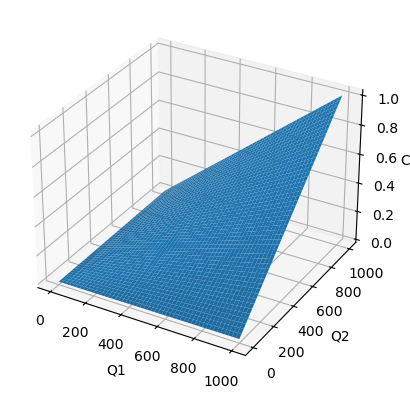
\includegraphics[keepaspectratio]{Session2Slides_files/figure-beamer/cell-31-output-1.png}}
\end{frame}

\begin{frame}
\end{frame}




\end{document}
